\section{Scatter Plots}
\subsection{Scatter Plots of Our Main Results}
\begin{figure}[H]
    \centering
    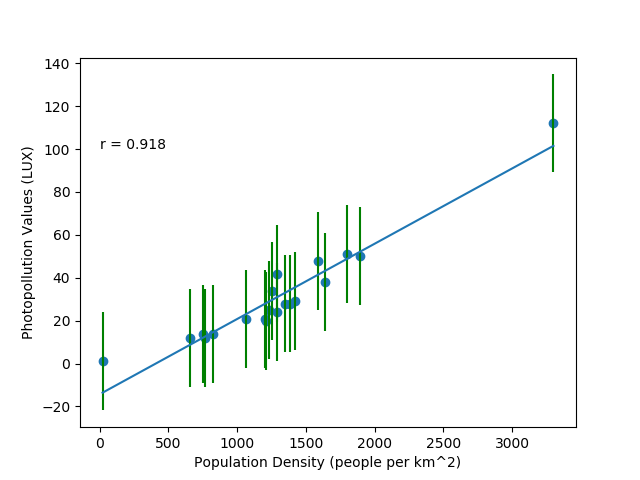
\includegraphics[width=.8\linewidth]{meanluxall}
    \caption{Mean Photopollution Values (All Sites)}
    \label{meanluxall}
\end{figure}
\begin{figure}[H]
    \centering
    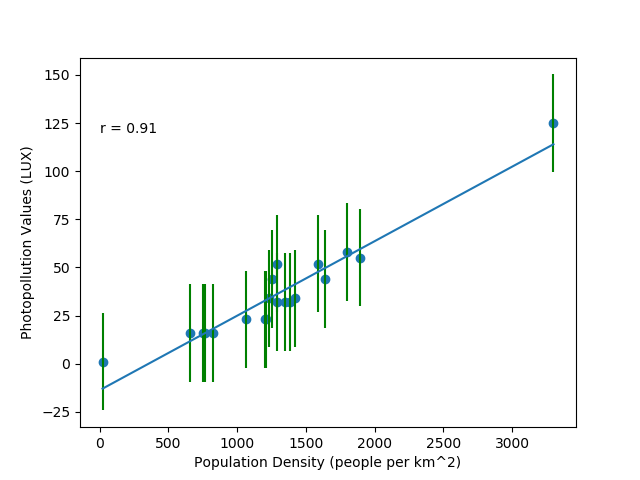
\includegraphics[width=.8\linewidth]{maxluxall}
    \caption{Max Photopollution Values (All Sites)}
    \label{maxluxall}
\end{figure}
\begin{figure}[H]
    \centering
    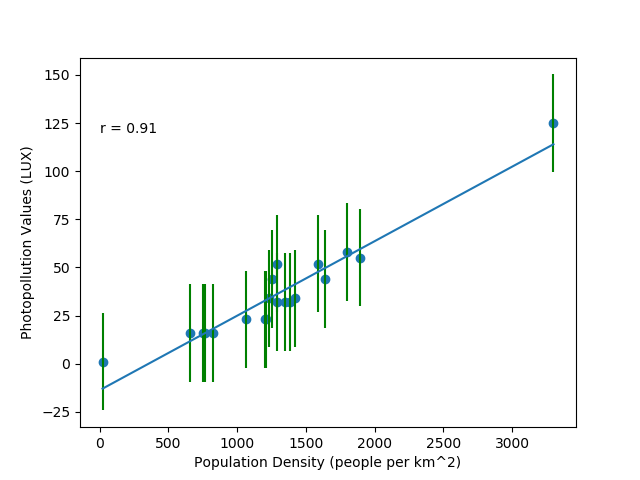
\includegraphics[width=.8\linewidth]{minluxall}
    \caption{Minimum Photopollution Values (All Sites)}
    \label{minluxall}
\end{figure}
\hfill
\subsection{Scatter Plots Based Results from Each County}
\begin{figure}[H]
    \centering
    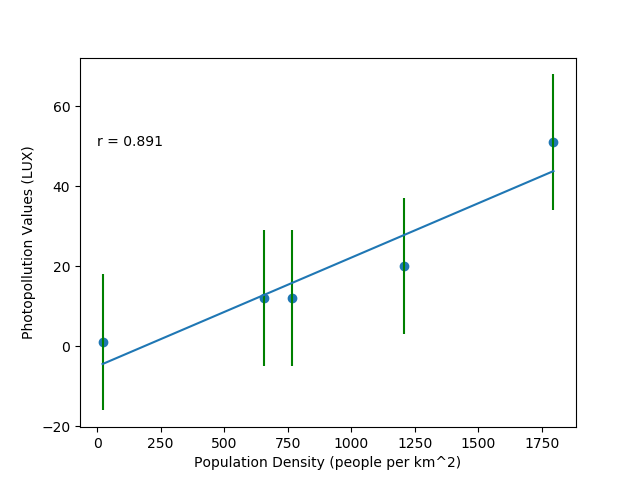
\includegraphics[width=.8\linewidth]{kerry}
    \caption{Kerry Photopollution Values}
    \label{kerry}
\end{figure}
\begin{figure}[H]
    \centering
    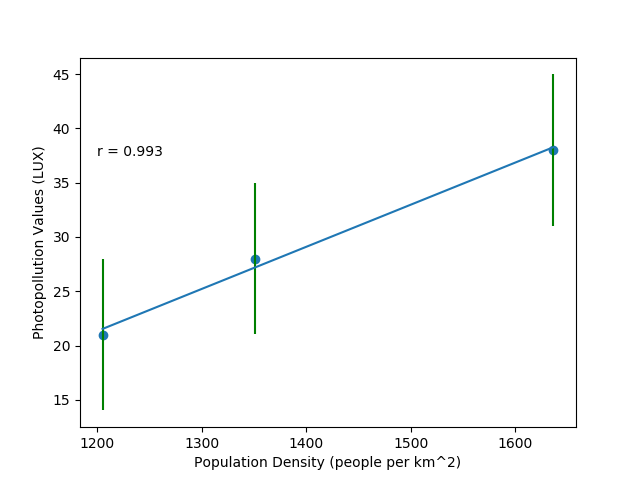
\includegraphics[width=.8\linewidth]{tipp}
    \caption{Tipperary Photopollution Values}
    \label{tipp}
\end{figure}
\hfill
\begin{figure}[H]
    \centering
    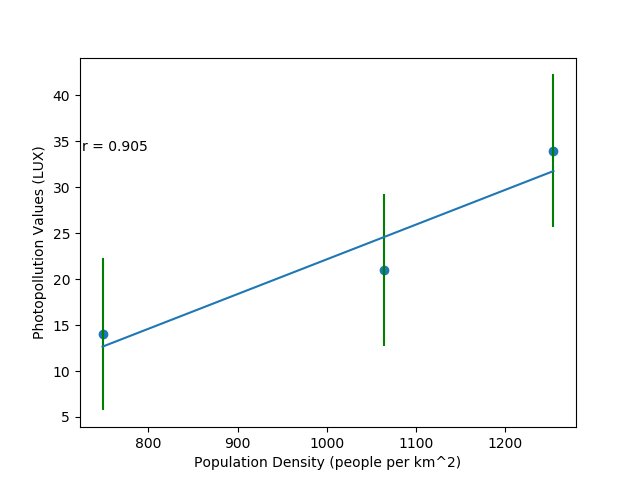
\includegraphics[width=.8\linewidth]{waterford}
    \caption{Waterford Photopollution Values}
    \label{waterford}
\end{figure}
\begin{figure}[H]
    \centering
    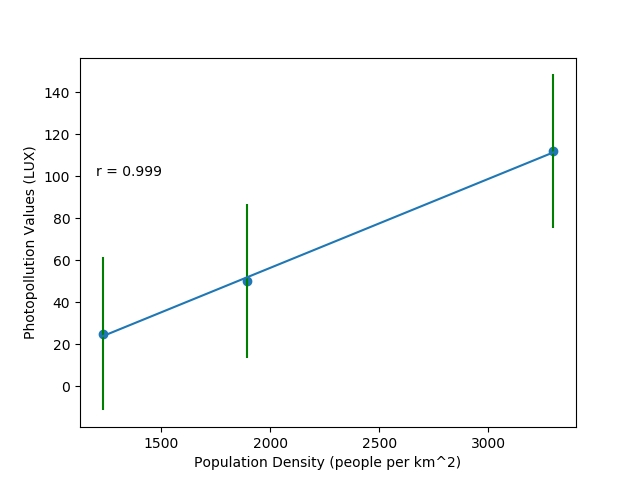
\includegraphics[width=.8\linewidth]{cork}
    \caption{Cork Photopollution Values}
    \label{cork}
\end{figure}
\hfill
\begin{figure}[H]
    \centering
    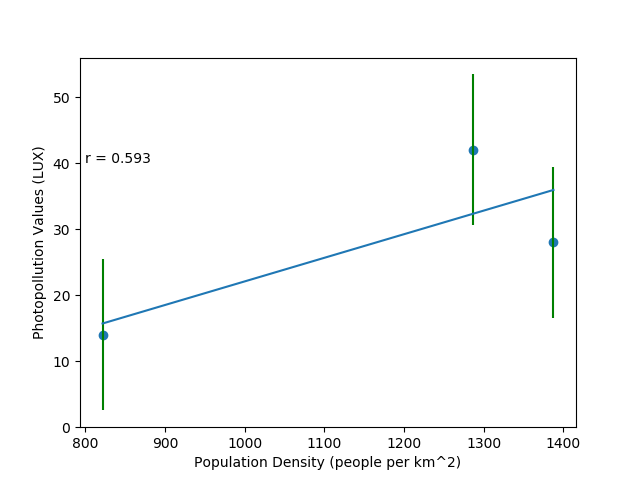
\includegraphics[width=.8\linewidth]{clare}
    \caption{Clare Photopollution Values}
    \label{clare}
\end{figure}
\begin{figure}[H]
    \centering
    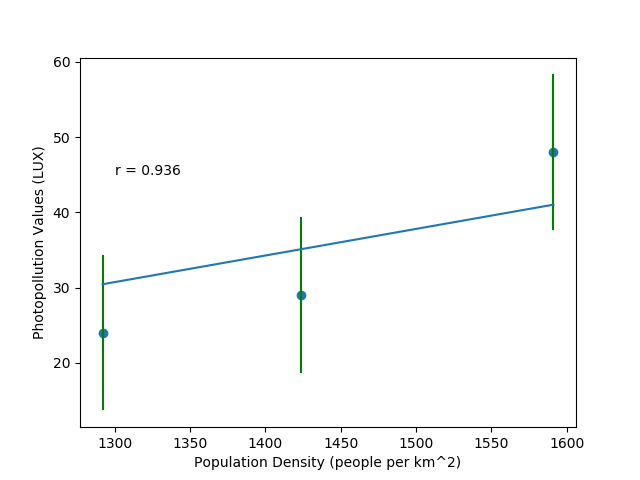
\includegraphics[width=.8\linewidth]{limerick}
    \caption{Limerick Photopollution Values}
    \label{limerick}
\end{figure}

\section{Mathematical Model}

\begin{equation}
\label{model} 
I = 0.03510566 d_x - 14.32414198 
\end{equation}

In this equation $I$ is the photopollution produced in that area, in the unit of measurement, $LUX$, and $d_x$ is the population density of that area (people per $km^{2}$). 

\hfill{}

\section{Grading System}
\begin{tabularx}{\textwidth}{|X|l|}
  \hline
  \textbf{LUX Value} & \textbf{Stargazing Conditions} \\ [25pt]
\hline
0 - 9 & Excellent Stargazing Conditions\\ [40pt]
\hline
9 - 17 & Good Stargazing Conditions\\ [40pt]
\hline
17 - 25 & Fair Stargazing Conditions\\ [40pt]
\hline
25 - 34 & Poor Stargazing Conditions\\ [40pt]
\hline
34 + & Terrible Stargazing Conditions\\ [40pt]
\hline
\end{tabularx}

\hfill

\section{Our Generated Maps}
\begin{figure}[H]
    \centering
    \caption{Maps generated in QGIS.}
    \label{qgis}
    \begin{subfigure}{\textwidth}
        \centering
        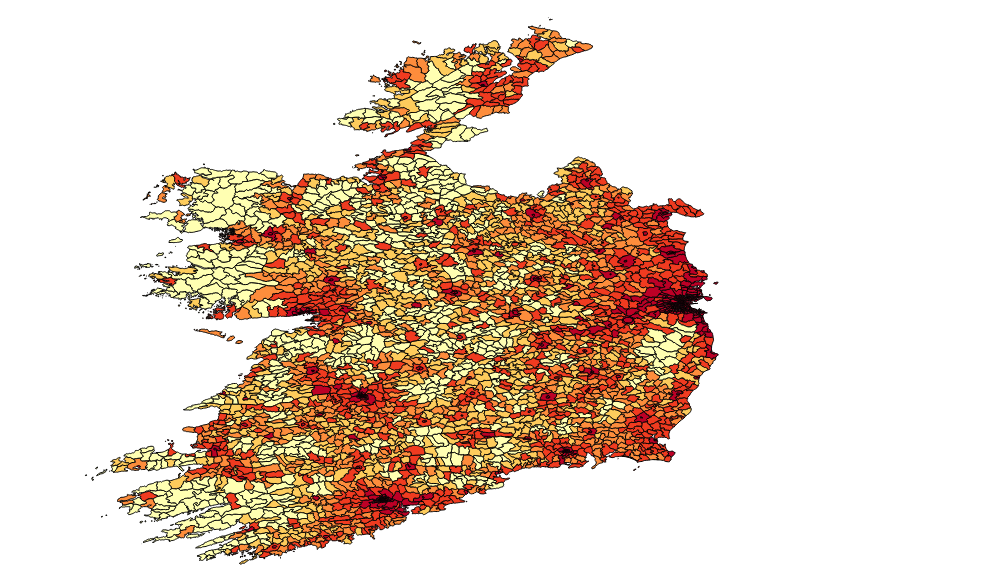
\includegraphics[width=\textwidth]{populationdensitymap}
        \caption{Our generated population density heat map of the Republic of Ireland}
        \label{pdheatmap}
    \end{subfigure}
    \hfill
    \begin{subfigure}{\textwidth}
        \centering
        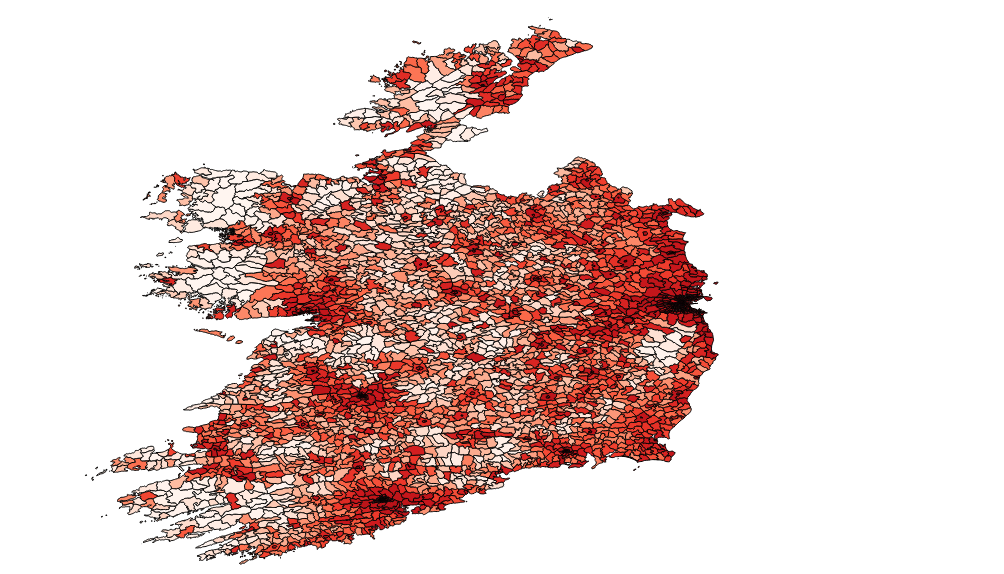
\includegraphics[width=\textwidth]{photopollutionmap}
        \caption{Our generated photopollution map of the Republic of Ireland}
        \label{photopollutionmap}
    \end{subfigure}
\end{figure}

\section{Nighttime Imagery of Ireland}
\begin{figure}[h]
    \centering
    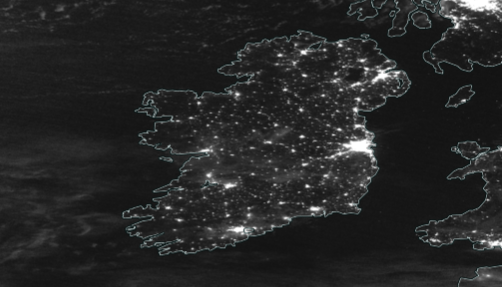
\includegraphics[width=\textwidth]{ireland}
    \caption{Nighttime Imagery of Ireland as provided by the VIIRS 2018 (March) Radiance.}
    \label{ireland}
\end{figure}